\documentclass[a4paper, 12pt]{report}

\usepackage[T1]{fontenc} % meilleures fontes pour les accents.
\usepackage[latin1]{inputenc} % utiliser à fond les claviers français
\usepackage[english]{babel}
\usepackage{graphicx}
\usepackage{subfigure}

% Infos
\title{GinkoTempo Application for iPhone}
\date{May 19, 2010}
\author{\textsc{S\'{e}bastien BARBIER} \and \textsc{Jocelyn FACCHINI}}

% Définition de nouvelles commandes

\begin{document}
	
\maketitle


\begin{abstract} 

In partnership with Ginko Besan\c{c}on, we developed an iPhone application that use their web service call Ginko tempo and optimise it for iPhone device. This was for us the opportunity to learn to develop an iPhone application, to use Objective-C and also to use the iPhone SDK.

We produced an application in accordance with Apple's ergonomics, with iPhone's look and feel, and which is pleasant to use. This project has been for us a great introduction on development for mobile device, and we tried to communicate our experience and enthusiasm in this present report.

\end{abstract}



\tableofcontents


\chapter{Introduction}

This project is conducted as part of our Master degree to apply our knowledges on a concrete case. We were free to choose our subject and which technology to study. We decided to take the Ginko project to worked on mobile device, in this case the iPhone.

During the few last years, the iPhone appeared as a totally new way of communication. There are more than 140 000 applications available today for this device which answers to every kind of needs. Ginko wants to create a mobile application for his service "GinkoTempo".

Ginko is a transport company in charge of Besan\c{c}on bus network. They built a web application called "GinkoTempo" \footnote{Available at the address http://www.ginkotempo.com } to have an instant access to the waiting time of every bus at a station. This application can freely be use with a simple internet connection but needed to be adapted for iPhone. In partnership with Ginko, our goal was to create an application to complete this offer.

This report is a presentation of our work. Chapter two introduce technology, tools and materials we used to develop this application. The Chapter trhee present our final product, the GinkoTempo application for iPhone. Finally, we will have a discussion about the future of this project, and briefly introduce some user feedback.


% Sur quoi on a travaillé
%Dans l'introduction ...

% Présentation de ce que l'on devait faire

\chapter{Tools and technology involved}

\section{Methodology and good practices}

% Method describes the steps you followed in conducting your work. This is useful for the reader to know how the methodology you used could have influenced your results.

The first step was to conduct an analysis of the subject. The objective was to completely understand users needs. To help us, an official from Ginko followed our development and has attended to all of our meetings. He was customer and defined all the technical specifications.

We first defined a list of functionalities based on a list of use-cases. Users have to be able to consult :

\begin{itemize}
	\item the waiting times of a station they know by name
	\item the waiting times of a station they will find from a specific bus line
	\item the waiting times of a station neir their GPS position
	\item the current traffic informations
\end{itemize}

But they also need to be able to :

\begin{itemize}
	\item create an user account
	\item consult station of their user account
	\item add and remove a station from their user account
\end{itemize}

Once completed, we immediately started to study tools we would have to work with. We studied two systems : iPhone and Android tools (iPhone OS\footnote{iPhone Operating System} SDK\footnote{Software Development Kit} and Android SDK) which are not using the same technologies. Because of the short time interval of time allocated to this project, we had to be efficient and decide how to start our development. We decided to start first with the iPhone OS and next to work on the Android one. 

This was not an easy task because iPhone OS is develop by Apple with Objective-C language. We both had no idea about how to use it, so we had to learn it. In comparison, Android's applications use Java language which has been studied during our lectures and would be more easy to start with. We decided to start the iPhone application because it is the most common platform and iPhone device was priority for Ginko.

Another difficulty was to communicate between our application and Ginko's server to access their databases. They developed a web-service which is an open access to data from the outside and they explained us how to use it.

Once those points had been resolved, we started our development.


\section{Material conditions}

To develop an iPhone application, it is required to use an Apple computer. In fact, iPhone development tools are only available on Mac OS X\footnote{Mac Computer Operating System}. Because the university does not have this kind of machine, we both had to use our personal laptop to do this.

As for our laptop, we both used our personnel mobile device, an "iPhone 3G" and an "HTC Magic" smartphone with Android. We only had one device of each type but this was not a real problem. In fact there is an application to simulate a mobile device and try our application directly on our computer. We only next discovered that iPhone OS simulator is a very light version of the OS and do not include some features as GPS or resources limitation. On the opposite, Android Simulator is way more efficient. 

Apple propose a complete set of softwares to help us in our development. We first learned to use Xcode which is an IDE \footnote{Integrated Development Environment} made by Apple to develop their own application. This IDE is delivered with "InterfaceBuilder" which is a wysiwyg\footnote{What You See Is What You Get} interface editor. If this solution first looks easy to use, we quickly realised that it would be harder to use than to learn how to make an interface programmatically. We also discovered "Instrument" application which is used to analyse and optimise the comportment of our project.

To access the Ginko's web service which use a protocol named soap, we had to find a software to create links between our application and their server. We discovered that the iPhone SDK don't manage natively this protocol, so we had to find a substitute. Because it is possible to execute C++ source code in an Objective-C project, we decided to use an external tool called gSoap. This tool is able to generate the structure need to communicate.

Finally, there is a specific policy to be allowed to develop on the iPhone OS. Ginko had to buy a license and define us as developers. Ginko gave us very quickly a certificate to install our application on our device and we could start developing and testing in real-life conditions.


\chapter{Application overview}



The iPhone development had been longer than expected. In fact, we had to learn how to use Objective-C and the iPhone SDK. Apple provides a complete documentation about both of them but in a very complex and technical english language.

At the end of this project, we haven't been able to start the Android development. There was too much work to be realised in a short period of time and so, we focused our development on the iPhone application. After eighteen weeks of work in parallels of our lectures, we finally obtained an application usable and quite efficient.


\section{Presentation of the application}

The main screen of application is the one with the waiting times (see Figure 3.1 (a)). For each bus line at a specific station, we display its number, colour, direction, and the waiting times for the next two bus - if there are available. This screen will be the main page which will be mainly consulted. If the use select a bus line, he can access some details as a bus description, eventually traffic informations relative to this specific line. Moreover, it is possible to add or remove this line from a user account - which will be explain later.


\subsection{List of stations}


Users can access to a list of all bus stations (see Figure 3.1 (b)). This is a list of station alphabetically ordered. Each station give an access to the waiting times of each lines.

\subsection{List of lines}


Users can access to a list of all lines (see Figure 3.1 (c)). This list is numerically ordered and give an access to the list of stations deserved by a chosen bus line.


\begin{figure}[htp]
  \centering
  \subfigure[List of stations]{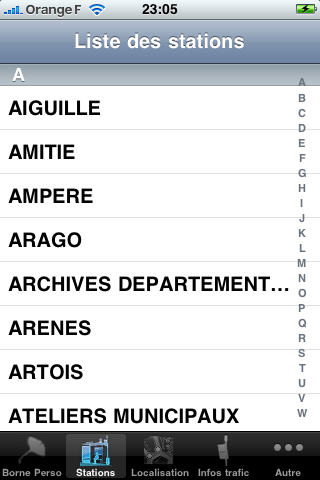
\includegraphics[scale=0.35]{images/stations}}                
  \subfigure[List of lines]{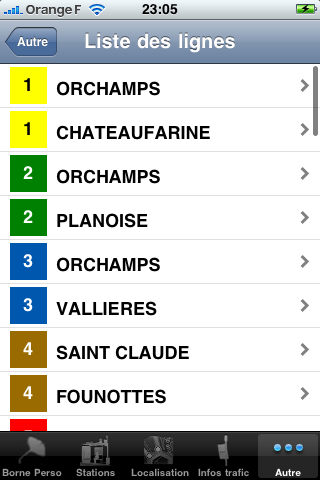
\includegraphics[scale=0.35]{images/lignes}}
  \subfigure[List of the waiting times]{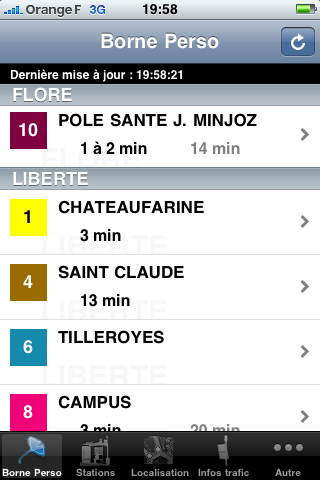
\includegraphics[scale=0.35]{images/borne}}

  \caption{Three different screens}
\end{figure}

\subsection{GPS Localisation}

Today, every new smartphone integrate a GPS to use localisation service. Users can use this functionality to find stations which are near to their current position (see Figure 3.2 (a)).


\subsection{Traffic informations}

Users can consult traffic informations about the Ginko Network directly from this page. Informations are displayed as a list of title (see Figure 3.1 (b)), if a user select one he can access to the complete message  (see Figure 3.2 (c)). Important messages are displayed in red and a counter is highlighted in all the application.



\subsection{User account}

Users can create a personal user account to save their favourite stations and have a quick access to them. They can use the application to create new account which can be used on our application and also on the GinkoTempo website. (see Figure 3.3 (a, b, c))

\begin{figure}[!hp]
  \centering
  \subfigure[GPS localisation]{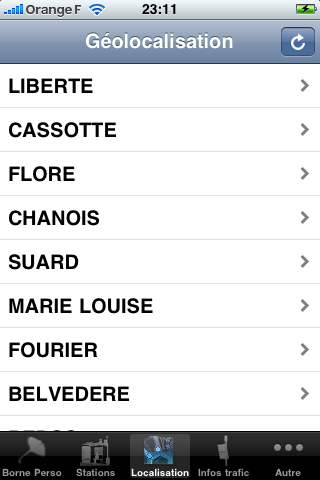
\includegraphics[scale=0.35]{images/localisation}}
  \subfigure[List of traffic info]{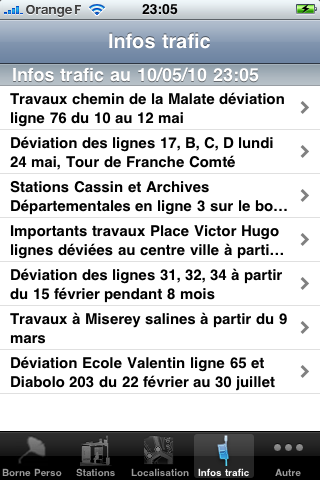
\includegraphics[scale=0.35]{images/traffic}}                
  \subfigure[Complete traffic info]{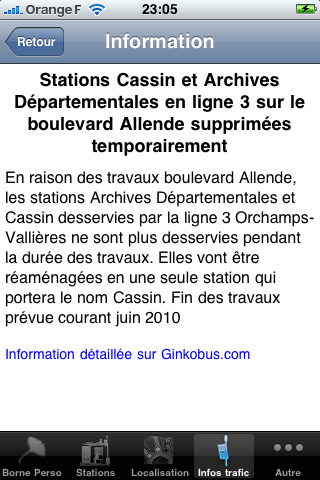
\includegraphics[scale=0.35]{images/traffic_full}}
  \caption{Traffic informations}
\end{figure}


\begin{figure}[!hp]
  \centering
  \subfigure[The waiting times of a user account]{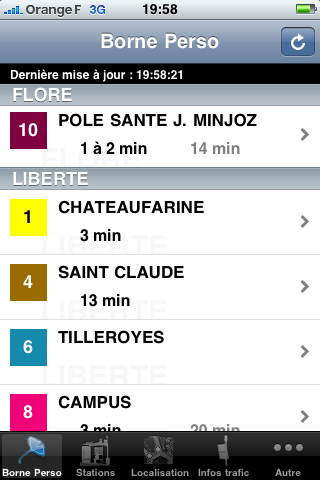
\includegraphics[scale=0.35]{images/borne}}                
  \subfigure[Details of a waiting times]{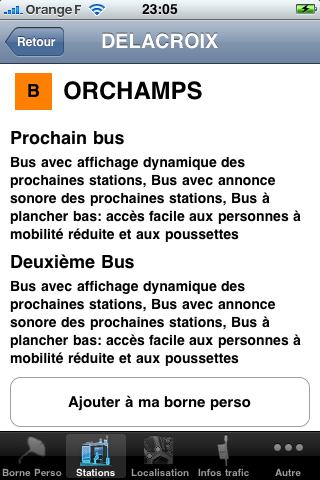
\includegraphics[scale=0.35]{images/details}}
  \subfigure[Setup a user account]{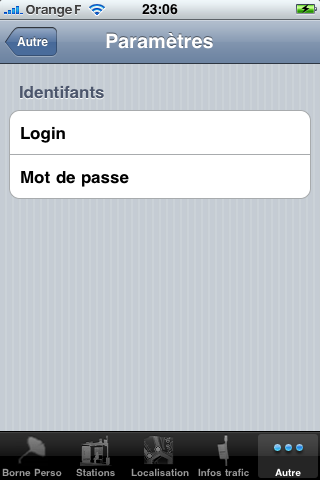
\includegraphics[scale=0.35]{images/login}}
  \caption{User account and management}
\end{figure}




% iPhone main Page, iPhone second page, iPhone third page.



% Discussion
\chapter{Discussion about our development}


\section{User Feedback} % (fold)

We took fifteen weeks to produce a first draft of the application. We only had few basic functionalities and didn't manage at all the user account, but had at this point some interesting results. We had to optimise the application to make it faster and user friendly. We worked a lot on the ergonomic to adopt the iPhone look and feel. This was one of the biggest key point because to make a good application, people need to feel comfortable with it.

Quickly in our development, we showed the application to some developers around us, and for most of them they had been able to use it instantly. They recognised a good integration with the iPhone, fluid interaction and most of all, a real simplicity. This was only a first and incomplete draft but results were encouraging.

When we implemented the user account functionality, the application reveals all his potential. For the first time, the application was completely functional and pleasant to use.

We didn't had enough time to realise a complete study but first feedbacks were really encouraging. This should be an interesting thing to do before starting to distribute it as an official application but we think everything is in place to have a good result.

\section{Regrets} % (fold)

The first topic of our subject was : Ginko Application for iPhone, Android and Windows Mobile. There was technically no way to implement a unique solution so we had to work on three different softwares. We first started with the most popular one ,the iPhone, but didn't had enough time to start another platform.

There is still some functionality to implement. A map with all bus stations could be possible to implement with the iPhone SDK. This could be a visual help to find a station and set an idea of the distance and the route to access it. It could be nice to implement a system alert. If an user need to take the bus, an alert warn him few minutes before. This could be relevant in some case, if you need 4 minutes to go to the bus station, you could optimise your route and save time.

A last thing, since we begin this product, a huge new product arrived on the market : the iPad. Even if our application is compatible with this device, our interface is optimised for small screen as the iPhone (3.5 in) and is not suitable for large screen (9.8 in). It could be comfortable to include in our application different visualisation mode depending on the device. Thanks to the structure of our application, it could be possible to do.

All points will be reported to Ginko and may be implemented in a future version of the application.

\chapter{Conclusion}

This project was an amazing subject for us. We were very enthusiastic about it and haven't been disappointed.

We had with this project the opportunity to work on a mobile device, and more specially the iPhone OS. Since few years, this is a hot topic because of the smartphones success. Working on this kind of project was a very interesting experience.

The university of Franche Comt\'{e} proposes a final year of Master Degree specialised in Networking and Mobile Computing where iPhone OS is studied. At the end of the year, we will have to choose a specialty and we thanks to this project will have a better idea of this option.


\end{document}